% 若编译失败,且生成 .synctex(busy) 辅助文件,可能有两个原因:
% 1. 需要插入的图片不存在:Ctrl + F 搜索 'figure' 将这些代码注释/删除掉即可
% 2. 路径/文件名含中文或空格:更改路径/文件名即可

% ------------------------------------------------------------- %
% >> ------------------ 文章宏包及相关设置 ------------------ << %
% 设定文章类型与编码格式
\documentclass[UTF8]{report}		

% 本文特殊宏包
\usepackage{siunitx} % 埃米单位

% 本 .tex 专属的宏定义
    \def\V{\ \mathrm{V}}
    \def\mV{\ \mathrm{mV}}
    \def\kV{\ \mathrm{KV}}
    \def\KV{\ \mathrm{KV}}
    \def\MV{\ \mathrm{MV}}
    \def\A{\ \mathrm{A}}
    \def\mA{\ \mathrm{mA}}
    \def\kA{\ \mathrm{KA}}
    \def\KA{\ \mathrm{KA}}
    \def\MA{\ \mathrm{MA}}
    \def\O{\ \Omega}
    \def\mO{\ \Omega}
    \def\kO{\ \mathrm{K}\Omega}
    \def\KO{\ \mathrm{K}\Omega}
    \def\MO{\ \mathrm{M}\Omega}
    \def\Hz{\ \mathrm{Hz}}

% 自定义宏定义
    \def\N{\mathbb{N}}
    \def\F{\mathbb{F}}
    \def\Z{\mathbb{Z}}
    \def\Q{\mathbb{Q}}
    \def\R{\mathbb{R}}
    \def\C{\mathbb{C}}
    \def\T{\mathbb{T}}
    \def\S{\mathbb{S}}
    \def\A{\mathbb{A}}
    \def\I{\mathscr{I}}
    \def\Im{\mathrm{Im\,}}
    \def\Re{\mathrm{Re\,}}
    \def\d{\mathrm{d}}
    \def\p{\partial}

% 导入基本宏包
    \usepackage[UTF8]{ctex}     % 设置文档为中文语言
    \usepackage[colorlinks, linkcolor=blue, anchorcolor=blue, citecolor=blue, urlcolor=blue]{hyperref}  % 宏包:自动生成超链接 (此宏包与标题中的数学环境冲突)
    % \usepackage{hyperref}  % 宏包:自动生成超链接 (此宏包与标题中的数学环境冲突)
    % \hypersetup{
    %     colorlinks=true,    % false:边框链接 ; true:彩色链接
    %     citecolor={blue},    % 文献引用颜色
    %     linkcolor={blue},   % 目录 (我们在目录处单独设置),公式,图表,脚注等内部链接颜色
    %     urlcolor={orange},    % 网页 URL 链接颜色,包括 \href 中的 text
    %     % cyan 浅蓝色 
    %     % magenta 洋红色
    %     % yellow 黄色
    %     % black 黑色
    %     % white 白色
    %     % red 红色
    %     % green 绿色
    %     % blue 蓝色
    %     % gray 灰色
    %     % darkgray 深灰色
    %     % lightgray 浅灰色
    %     % brown 棕色
    %     % lime 石灰色
    %     % olive 橄榄色
    %     % orange 橙色
    %     % pink 粉红色
    %     % purple 紫色
    %     % teal 蓝绿色
    %     % violet 紫罗兰色
    % }

    % \usepackage{docmute}    % 宏包:子文件导入时自动去除导言区,用于主/子文件的写作方式,\include{./51单片机笔记}即可。注:启用此宏包会导致.tex文件capacity受限。
    \usepackage{amsmath}    % 宏包:数学公式
    \usepackage{mathrsfs}   % 宏包:提供更多数学符号
    \usepackage{amssymb}    % 宏包:提供更多数学符号
    \usepackage{pifont}     % 宏包:提供了特殊符号和字体
    \usepackage{extarrows}  % 宏包:更多箭头符号
    \usepackage{multicol}   % 宏包:支持多栏 
    \usepackage{graphicx}   % 宏包:插入图片
    \usepackage{float}      % 宏包:设置图片浮动位置
    %\usepackage{article}    % 宏包:使文本排版更加优美
    \usepackage{tikz}       % 宏包:绘图工具
    %\usepackage{pgfplots}   % 宏包:绘图工具
    \usepackage{enumerate}  % 宏包:列表环境设置
    \usepackage{enumitem}   % 宏包:列表环境设置

% 文章页面margin设置
    \usepackage[a4paper]{geometry}
        \geometry{top=1in}
        \geometry{bottom=1in}
        \geometry{left=0.75in}
        \geometry{right=0.75in}   % 设置上下左右页边距
        \geometry{marginparwidth=1.75cm}    % 设置边注距离(注释、标记等)

% 定义 solution 环境
\usepackage{amsthm}
\newtheorem{solution}{Solution}
        \geometry{bottom=1in}
        \geometry{left=0.75in}
        \geometry{right=0.75in}   % 设置上下左右页边距
        \geometry{marginparwidth=1.75cm}    % 设置边注距离(注释、标记等)

% 配置数学环境
    \usepackage{amsthm} % 宏包:数学环境配置
    % theorem-line 环境自定义
        \newtheoremstyle{MyLineTheoremStyle}% <name>
            {11pt}% <space above>
            {11pt}% <space below>
            {}% <body font> 使用默认正文字体
            {}% <indent amount>
            {\bfseries}% <theorem head font> 设置标题项为加粗
            {:}% <punctuation after theorem head>
            {.5em}% <space after theorem head>
            {\textbf{#1}\thmnumber{#2}\ \ (\,\textbf{#3}\,)}% 设置标题内容顺序
        \theoremstyle{MyLineTheoremStyle} % 应用自定义的定理样式
        \newtheorem{LineTheorem}{Theorem.\,}
    % theorem-block 环境自定义
        \newtheoremstyle{MyBlockTheoremStyle}% <name>
            {11pt}% <space above>
            {11pt}% <space below>
            {}% <body font> 使用默认正文字体
            {}% <indent amount>
            {\bfseries}% <theorem head font> 设置标题项为加粗
            {:\\ \indent}% <punctuation after theorem head>
            {.5em}% <space after theorem head>
            {\textbf{#1}\thmnumber{#2}\ \ (\,\textbf{#3}\,)}% 设置标题内容顺序
        \theoremstyle{MyBlockTheoremStyle} % 应用自定义的定理样式
        \newtheorem{BlockTheorem}[LineTheorem]{Theorem.\,} % 使用 LineTheorem 的计数器
    % definition 环境自定义
        \newtheoremstyle{MySubsubsectionStyle}% <name>
            {11pt}% <space above>
            {11pt}% <space below>
            {}% <body font> 使用默认正文字体
            {}% <indent amount>
            {\bfseries}% <theorem head font> 设置标题项为加粗
           % {:\\ \indent}% <punctuation after theorem head>
            {\\\indent}
            {0pt}% <space after theorem head>
            {\textbf{#3}}% 设置标题内容顺序
        \theoremstyle{MySubsubsectionStyle} % 应用自定义的定理样式
        \newtheorem{definition}{}

%宏包:有色文本框(proof环境)及其设置
    \usepackage[dvipsnames,svgnames]{xcolor}    %设置插入的文本框颜色
    \usepackage[strict]{changepage}     % 提供一个 adjustwidth 环境
    \usepackage{framed}     % 实现方框效果
        \definecolor{graybox_color}{rgb}{0.95,0.95,0.96} % 文本框颜色。修改此行中的 rgb 数值即可改变方框纹颜色,具体颜色的rgb数值可以在网站https://colordrop.io/ 中获得。(截止目前的尝试还没有成功过,感觉单位不一样)(找到喜欢的颜色,点击下方的小眼睛,找到rgb值,复制修改即可)
        \newenvironment{graybox}{%
        \def\FrameCommand{%
        \hspace{1pt}%
        {\color{gray}\small \vrule width 2pt}%
        {\color{graybox_color}\vrule width 4pt}%
        \colorbox{graybox_color}%
        }%
        \MakeFramed{\advance\hsize-\width\FrameRestore}%
        \noindent\hspace{-4.55pt}% disable indenting first paragraph
        \begin{adjustwidth}{}{7pt}%
        \vspace{2pt}\vspace{2pt}%
        }
        {%
        \vspace{2pt}\end{adjustwidth}\endMakeFramed%
        }



% 外源代码插入设置
    % matlab 代码插入设置
    \usepackage{matlab-prettifier}
        \lstset{style=Matlab-editor}    % 继承 matlab 代码高亮 , 此行不能删去
    \usepackage[most]{tcolorbox} % 引入tcolorbox包 
    \usepackage{listings} % 引入listings包
        \tcbuselibrary{listings, skins, breakable}
        \newfontfamily\codefont{Consolas} % 定义需要的 codefont 字体
        \lstdefinestyle{MatlabStyle_inc}{   % 插入代码的样式
            language=Matlab,
            basicstyle=\small\ttfamily\codefont,    % ttfamily 确保等宽 
            breakatwhitespace=false,
            breaklines=true,
            captionpos=b,
            keepspaces=true,
            numbers=left,
            numbersep=15pt,
            showspaces=false,
            showstringspaces=false,
            showtabs=false,
            tabsize=2,
            xleftmargin=15pt,   % 左边距
            %frame=single, % single 为包围式单线框
            frame=shadowbox,    % shadowbox 为带阴影包围式单线框效果
            %escapeinside=``,   % 允许在代码块中使用 LaTeX 命令 (此行无用)
            %frameround=tttt,    % tttt 表示四个角都是圆角
            framextopmargin=0pt,    % 边框上边距
            framexbottommargin=0pt, % 边框下边距
            framexleftmargin=5pt,   % 边框左边距
            framexrightmargin=5pt,  % 边框右边距
            rulesepcolor=\color{red!20!green!20!blue!20}, % 阴影框颜色设置
            %backgroundcolor=\color{blue!10}, % 背景颜色
        }
        \lstdefinestyle{MatlabStyle_src}{   % 插入代码的样式
            language=Matlab,
            basicstyle=\small\ttfamily\codefont,    % ttfamily 确保等宽 
            breakatwhitespace=false,
            breaklines=true,
            captionpos=b,
            keepspaces=true,
            numbers=left,
            numbersep=15pt,
            showspaces=false,
            showstringspaces=false,
            showtabs=false,
            tabsize=2,
        }
        \newtcblisting{matlablisting}{
            %arc=2pt,        % 圆角半径
            % 调整代码在 listing 中的位置以和引入文件时的格式相同
            top=0pt,
            bottom=0pt,
            left=-5pt,
            right=-5pt,
            listing only,   % 此句不能删去
            listing style=MatlabStyle_src,
            breakable,
            colback=white,   % 选一个合适的颜色
            colframe=black!0,   % 感叹号后跟不透明度 (为 0 时完全透明)
        }
        \lstset{
            style=MatlabStyle_inc,
        }



% table 支持
    \usepackage{booktabs}   % 宏包:三线表
    %\usepackage{tabularray} % 宏包:表格排版
    %\usepackage{longtable}  % 宏包:长表格
    %\usepackage[longtable]{multirow} % 宏包:multi 行列


% figure 设置
\usepackage{graphicx}   % 支持 jpg, png, eps, pdf 图片 
\usepackage{float}      % 支持 H 选项
\usepackage{svg}        % 支持 svg 图片
\usepackage{subcaption} % 支持子图
\svgsetup{
        % 指向 inkscape.exe 的路径
       inkscapeexe = C:/aa_MySame/inkscape/bin/inkscape.exe, 
        % 一定程度上修复导入后图片文字溢出几何图形的问题
       inkscapelatex = false                 
   }

% 图表进阶设置
    \usepackage{caption}    % 图注、表注
        \captionsetup[figure]{name=图}  
        \captionsetup[table]{name=表}
        \captionsetup{
            labelfont=bf, % 设置标签为粗体
            textfont=bf,  % 设置文本为粗体
            font=small  
        }
    \usepackage{float}     % 图表位置浮动设置 
        % \floatstyle{plaintop} % 设置表格标题在表格上方
        % \restylefloat{table}  % 应用设置


% 圆圈序号自定义
    \newcommand*\circled[1]{\tikz[baseline=(char.base)]{\node[shape=circle,draw,inner sep=0.8pt, line width = 0.03em] (char) {\small \bfseries #1};}}   % TikZ solution


% 列表设置
    \usepackage{enumitem}   % 宏包:列表环境设置
        \setlist[enumerate]{
            label=\bfseries(\arabic*) ,   % 设置序号样式为加粗的 (1) (2) (3)
            ref=\arabic*, % 如果需要引用列表项,这将决定引用格式(这里仍然使用数字)
            itemsep=0pt, parsep=0pt, topsep=0pt, partopsep=0pt, leftmargin=3.5em} 
        \setlist[itemize]{itemsep=0pt, parsep=0pt, topsep=0pt, partopsep=0pt, leftmargin=3.5em}
        \newlist{circledenum}{enumerate}{1} % 创建一个新的枚举环境  
        \setlist[circledenum,1]{  
            label=\protect\circled{\arabic*}, % 使用 \arabic* 来获取当前枚举计数器的值,并用 \circled 包装它  
            ref=\arabic*, % 如果需要引用列表项,这将决定引用格式(这里仍然使用数字)
            itemsep=0pt, parsep=0pt, topsep=0pt, partopsep=0pt, leftmargin=3.5em
        }  

% 文章默认字体设置
    \usepackage{fontspec}   % 宏包:字体设置
        \setmainfont{STKaiti}    % 设置中文字体为宋体字体
        \setCJKmainfont[AutoFakeBold=3]{STKaiti} % 设置加粗字体为 STKaiti 族,AutoFakeBold 可以调整字体粗细
        \setmainfont{Times New Roman} % 设置英文字体为Times New Roman


% 其它设置
    % 脚注设置
    \renewcommand\thefootnote{\ding{\numexpr171+\value{footnote}}}
    % 参考文献引用设置
        \bibliographystyle{unsrt}   % 设置参考文献引用格式为unsrt
        \newcommand{\upcite}[1]{\textsuperscript{\cite{#1}}}     % 自定义上角标式引用
    % 文章序言设置
        \newcommand{\cnabstractname}{序言}
        \newenvironment{cnabstract}{%
            \par\Large
            \noindent\mbox{}\hfill{\bfseries \cnabstractname}\hfill\mbox{}\par
            \vskip 2.5ex
            }{\par\vskip 2.5ex}


% 各级标题自定义设置
    \usepackage{titlesec}   
    % chapter
        \titleformat{\chapter}[hang]{\normalfont\Large\bfseries\centering}{题目}{10pt}{}
        \titlespacing*{\chapter}{0pt}{-30pt}{10pt} % 控制上方空白的大小
    % section
        \titleformat{\section}[hang]{\normalfont\large\bfseries}{\thesection}{8pt}{}
    % subsection
        %\titleformat{\subsubsection}[hang]{\normalfont\bfseries}{}{8pt}{}
    % subsubsection
        %\titleformat{\subsubsection}[hang]{\normalfont\bfseries}{}{8pt}{}

% 见到的一个有意思的对于公式中符号的彩色解释的环境
        \usepackage[dvipsnames]{xcolor}
        \usepackage{tikz}
        \usetikzlibrary{backgrounds}
        \usetikzlibrary{arrows,shapes}
        \usetikzlibrary{tikzmark}
        \usetikzlibrary{calc}
        
        \usepackage{amsmath}
        \usepackage{amsthm}
        \usepackage{amssymb}
        \usepackage{mathtools, nccmath}
        \usepackage{wrapfig}
        \usepackage{comment}
        
        % To generate dummy text
        \usepackage{blindtext}
        
        
        %color
        %\usepackage[dvipsnames]{xcolor}
        % \usepackage{xcolor}
        
        
        %\usepackage[pdftex]{graphicx}
        \usepackage{graphicx}
        % declare the path(s) for graphic files
        %\graphicspath{{../Figures/}}
        
        % extensions so you won't have to specify these with
        % every instance of \includegraphics
        % \DeclareGraphicsExtensions{.pdf,.jpeg,.png}
        
        % for custom commands
        \usepackage{xspace}
        
        % table alignment
        \usepackage{array}
        \usepackage{ragged2e}
        \newcolumntype{P}[1]{>{\RaggedRight\hspace{0pt}}p{#1}}
        \newcolumntype{X}[1]{>{\RaggedRight\hspace*{0pt}}p{#1}}
        
        % color box
        \usepackage{tcolorbox}
        
        
        % for tikz
        \usepackage{tikz}
        %\usetikzlibrary{trees}
        \usetikzlibrary{arrows,shapes,positioning,shadows,trees,mindmap}
        \usetikzlibrary{graphs} % <-- Added for \graph syntax
        % \usepackage{forest}
        \usepackage[edges]{forest}
        \usetikzlibrary{arrows.meta}
        \colorlet{linecol}{black!75}
        \usepackage{xkcdcolors} % xkcd colors
        
        
        % for colorful equation
        \usepackage{tikz}
        \usetikzlibrary{backgrounds}
        \usetikzlibrary{arrows,shapes}
        \usetikzlibrary{tikzmark}
        \usetikzlibrary{calc}
        % Commands for Highlighting text -- non tikz method
        \newcommand{\highlight}[2]{\colorbox{#1!17}{$\displaystyle #2$}}
        %\newcommand{\highlight}[2]{\colorbox{#1!17}{$#2$}}
        \newcommand{\highlightdark}[2]{\colorbox{#1!47}{$\displaystyle #2$}}
        
        % my custom colors for shading
        \colorlet{mhpurple}{Plum!80}
        
        
        % Commands for Highlighting text -- non tikz method
        \renewcommand{\highlight}[2]{\colorbox{#1!17}{#2}}
        \renewcommand{\highlightdark}[2]{\colorbox{#1!47}{#2}}
        
        % Some math definitions
        \newcommand{\lap}{\mathrm{Lap}}
        \newcommand{\pr}{\mathrm{Pr}}
        
        \newcommand{\Tset}{\mathcal{T}}
        \newcommand{\Dset}{\mathcal{D}}
        \newcommand{\Rbound}{\widetilde{\mathcal{R}}}

% >> ------------------ 文章宏包及相关设置 ------------------ << %
% ------------------------------------------------------------- %



% ----------------------------------------------------------- %
% >> --------------------- 文章信息区 --------------------- << %
% 页眉页脚设置

\usepackage{fancyhdr}   %宏包:页眉页脚设置
    \pagestyle{fancy}
    \fancyhf{}
    \cfoot{\thepage}
    \renewcommand\headrulewidth{1pt}
    \renewcommand\footrulewidth{0pt}
    \rhead{数据结构与算法期末复习,\ 尹超,\ 2023K8009926003}
    \lhead{Homework}


%文档信息设置
\title{数据结构与算法期末复习\\ Homework}
\author{尹超\\ \footnotesize 中国科学院大学,北京 100049\\ Carter Yin \\ \footnotesize University of Chinese Academy of Sciences, Beijing 100049, China}
\date{\footnotesize 2024.8 -- 2025.1}
% >> --------------------- 文章信息区 --------------------- << %
% ----------------------------------------------------------- %     


% 开始编辑文章

% 定义 tikz 样式 splaynode 和 highlight
\tikzset{
  splaynode/.style={draw, circle, minimum size=7mm, inner sep=0pt},
  highlight/.style={draw, circle, minimum size=7mm, inner sep=0pt, fill=yellow!30}
}

\begin{document}
\zihao{5}           % 设置全文字号大小

% --------------------------------------------------------------- %
% >> --------------------- 封面序言与目录 --------------------- << %
% 封面
    \maketitle\newpage  
    \pagenumbering{Roman} % 页码为大写罗马数字
    \thispagestyle{fancy}   % 显示页码、页眉等

% 序言
    \begin{cnabstract}\normalsize 
        本文为笔者数据结构与算法的期末复习笔记。\par
        望老师批评指正。
    \end{cnabstract}
    \addcontentsline{toc}{chapter}{序言} % 手动添加为目录

% % 不换页目录
%     \setcounter{tocdepth}{0}
%     \noindent\rule{\textwidth}{0.1em}   % 分割线
%     \noindent\begin{minipage}{\textwidth}\centering 
%         \vspace{1cm}
%         \tableofcontents\thispagestyle{fancy}   % 显示页码、页眉等   
%     \end{minipage}  
%     \addcontentsline{toc}{chapter}{目录} % 手动添加为目录

% 目录
\setcounter{tocdepth}{4}                % 目录深度(为1时显示到section)
\tableofcontents                        % 目录页
\addcontentsline{toc}{chapter}{目录}    % 手动添加此页为目录
\thispagestyle{fancy}                   % 显示页码、页眉等 

% 收尾工作
    \newpage    
    \pagenumbering{arabic} 

% >> --------------------- 封面序言与目录 --------------------- << %
% --------------------------------------------------------------- %

\chapter{第十一章 优先级队列}

\section*{181}
\begin{graybox}
完全二叉堆中父节点的优先级
A. 不小于它的孩子
B. 不等于它的孩子
C. 和它的孩子没有必然的大小关系
D. 等于它的孩子
\end{graybox}

\begin{solution}
正确答案是 A。

\textbf{详细分析:}

二叉堆(Binary Heap)是一种特殊的完全二叉树,它满足\textbf{堆序性质(Heap Property)}。堆序性质分为两种:

\begin{enumerate}
    \item \textbf{最大堆(Max-Heap):}
    对于堆中任意一个节点,其优先级(或键值)都\textbf{大于或等于}其子节点的优先级。即 `parent.priority >= child.priority`。在这种情况下,父节点的优先级\textbf{不小于}它的孩子。

    \item \textbf{最小堆(Min-Heap):}
    对于堆中任意一个节点,其优先级(或键值)都\textbf{小于或等于}其子节点的优先级。即 `parent.priority <= child.priority`。在这种情况下,父节点的优先级\textbf{不大于}它的孩子。
\end{enumerate}

题目中没有明确指出是最大堆还是最小堆,但通常在讨论“优先级”时,默认指的是数值越大优先级越高,这对应于最大堆的性质。

\textbf{分析选项:}
\begin{itemize}
    \item \textbf{A. 不小于它的孩子:} 这准确地描述了最大堆的性质。
    \item \textbf{B. 不等于它的孩子:} 错误。在堆中,父子节点的优先级可以相等。
    \item \textbf{C. 和它的孩子没有必然的大小关系:} 错误。堆序性质本身就是一种严格的大小关系。
    \item \textbf{D. 等于它的孩子:} 错误。这只是一种特殊情况,不是普遍性质。
\end{itemize}

因此,选项A是描述二叉堆(特别是最大堆)性质的最准确的选项。
\end{solution}

\section*{182}
\begin{graybox}
在完全二叉堆中插入元素的方法是
A. 插入到底层,上滤
B. 插入到根节点,下滤
C. 直接插入到底层
D. 直接插入到根节点
\end{graybox}

\begin{solution}
正确答案是 A。

\textbf{详细分析:}

在完全二叉堆中插入一个新元素,必须同时满足两个条件:
\begin{enumerate}
    \item \textbf{结构性:} 插入后,树必须仍然是一棵\textbf{完全二叉树}。
    \item \textbf{堆序性:} 插入后,所有节点必须满足\textbf{堆序性质}(即父节点的优先级不小于/不大于其子节点)。
\end{enumerate}

正确的插入操作遵循以下两步:

\begin{enumerate}
    \item \textbf{插入到底层:} 为了维持完全二叉树的结构,新元素必须被放置在树的最后一个位置,即从左到右的第一个可用空位上。这通常是在数组表示的末尾添加该元素。这一步满足了“结构性”。

    \item \textbf{上滤(Percolate Up / Sift Up):} 插入新元素后,可能会破坏堆序性(例如,新元素的优先级可能高于其父节点)。因此,需要将新元素与其父节点进行比较。如果新元素的优先级更高(在最大堆中),则与父节点交换位置。这个过程不断重复,将新元素沿着路径向根节点方向“上滤”,直到它找到一个优先级不低于它的父节点,或者它自己成为根节点为止。这一步恢复了“堆序性”。
\end{enumerate}

\textbf{其他选项分析:}
\begin{itemize}
    \item \textbf{B. 插入到根节点,下滤:} “下滤”(Percolate Down)操作通常用于删除堆顶元素(`deleteMax`或`deleteMin`)后的调整过程,而不是插入。
    \item \textbf{C. 直接插入到底层:} 这只完成了第一步,没有执行恢复堆序性的“上滤”操作,是不完整的。
    \item \textbf{D. 直接插入到根节点:} 这会破坏完全二叉树的结构(除非堆为空)。
\end{itemize}
\end{solution}


\section*{183}
\begin{graybox}
规模为n的完全二叉堆中插入元素的时间复杂
度为:
A. O(nlogn)
B. O(n)
C. O(logn)
D. O(1)
\end{graybox}

\begin{solution}
正确答案是 C。

\textbf{详细分析:}

\begin{enumerate}
    \item \textbf{插入操作回顾:}
    在完全二叉堆中插入一个元素包含两个步骤:
    \begin{itemize}
        \item 将新元素添加到堆的末尾(即完全二叉树的下一个可用位置)。这个操作本身是 $O(1)$。
        \item 对新插入的元素执行“上滤”(Percolate Up)操作,以恢复堆序性。
    \end{itemize}

    \item \textbf{上滤操作的复杂度:}
    \begin{itemize}
        \item “上滤”操作是将新元素与其父节点比较,如果需要则交换,然后继续向上与新的父节点比较,直到找到合适的位置或到达根节点。
        \item 这个过程所经过的路径长度,在最坏情况下,是从堆的最低层一直到根节点。
        \item 这个路径的长度等于或小于堆的高度。
    \end{itemize}

    \item \textbf{完全二叉堆的高度:}
    一个包含 `n` 个节点的完全二叉树,其高度 `h` 约为 $\log_2 n$。更准确地说,高度是 $\lfloor \log_2 n \rfloor$。

    \item \textbf{结论:}
    由于“上滤”操作的执行次数最多等于堆的高度,因此在规模为 `n` 的完全二叉堆中插入一个元素的时间复杂度由堆的高度决定,即 $O(\log n)$。
\end{enumerate}

\textbf{其他选项分析:}
\begin{itemize}
    \item \textbf{A. O(nlogn):} 这通常是堆排序(HeapSort)的复杂度,或者是通过逐个插入 `n` 个元素来构建一个堆的复杂度。
    \item \textbf{B. O(n):} 这是通过“自底向上”的`heapify`算法批量建堆的复杂度。
    \item \textbf{D. O(1):} 这是插入操作的理想情况(新元素不需要上滤),但不是最坏情况下的时间复杂度。
\end{itemize}
\end{solution}


\section*{184}
\begin{graybox}
完全二叉堆中要删除一个元素时,这个元
素的位置是:
A. 根节点
B. 叶子节点
C. 可以是任意节点
D. 根节点或叶子节点
\end{graybox}

\begin{solution}
正确答案是 A。

\textbf{详细分析:}

\begin{enumerate}
    \item \textbf{堆作为优先队列:}
    完全二叉堆最主要的应用是作为\textbf{优先队列(Priority Queue)}。优先队列的核心操作之一就是取出并删除具有最高(或最低)优先级的元素。

    \item \textbf{堆序性质:}
    根据堆序性质,具有最高优先级的元素(在最大堆中)或最低优先级的元素(在最小堆中)总是位于堆的\textbf{根节点}。

    \item \textbf{删除操作(`deleteMax` 或 `deleteMin`):}
    因此,堆的标准删除操作总是删除\textbf{根节点}的元素。其具体步骤如下:
    \begin{itemize}
        \item \textbf{保存根节点:} 先将根节点的元素值保存下来,作为返回值。
        \item \textbf{替换根节点:} 将堆中最后一个元素(即完全二叉树最底层最右边的叶子节点)移动到根节点的位置。这一步是为了维持完全二叉树的结构。
        \item \textbf{下滤(Percolate Down):} 将新的根节点与其子节点比较,如果它的优先级低于其子节点(在最大堆中),则与优先级最高的子节点交换。这个过程不断重复,将该元素沿着路径向叶子节点方向“下滤”,直到它找到一个位置,使得它的优先级不低于其子节点,或者它自己成为叶子节点。这一步是为了恢复堆序性。
    \end{itemize}
\end{enumerate}

\textbf{其他选项分析:}
\begin{itemize}
    \item \textbf{B. 叶子节点:} 叶子节点不是被删除的目标,而是用来填补根节点空缺的“替补队员”。
    \item \textbf{C. 可以是任意节点:} 虽然技术上可以实现删除任意位置的元素(通过类似的方法),但这并不是堆的标准和高效操作。堆的设计初衷就是为了高效地访问和删除根节点。
    \item \textbf{D. 根节点或叶子节点:} 删除操作只针对根节点。
\end{itemize}
\end{solution}

\section*{185}
\begin{graybox}
规模为n的完全二叉堆中删除元素的时间复杂
度为:
A. O(nlogn)
B. O(n)
C. O(logn)
D. O(1)
\end{graybox}

\begin{solution}
正确答案是 C。

\textbf{详细分析:}

\begin{enumerate}
    \item \textbf{删除操作回顾:}
    在完全二叉堆中删除元素(特指删除根节点,即`deleteMax`或`deleteMin`)包含以下步骤:
    \begin{itemize}
        \item 移除根节点元素。
        \item 将堆的最后一个元素(位于最底层最右侧)移动到根节点位置。此操作为 $O(1)$。
        \item 对新的根节点执行“下滤”(Percolate Down)操作,以恢复堆序性。
    \end{itemize}

    \item \textbf{下滤操作的复杂度:}
    \begin{itemize}
        \item “下滤”操作是将新的根节点与其子节点比较,如果需要则与优先级更高的子节点交换,然后继续向下与新的子节点比较,直到找到合适的位置或成为叶子节点。
        \item 这个过程所经过的路径长度,在最坏情况下,是从根节点一直到堆的最低层。
        \item 这个路径的长度等于或小于堆的高度。
    \end{itemize}

    \item \textbf{完全二叉堆的高度:}
    一个包含 `n` 个节点的完全二叉树,其高度 `h` 约为 $\log_2 n$。

    \item \textbf{结论:}
    由于“下滤”操作是删除过程中的主导步骤,其执行次数最多等于堆的高度,因此在规模为 `n` 的完全二叉堆中删除一个元素的时间复杂度由堆的高度决定,即 $O(\log n)$。
\end{enumerate}

\textbf{其他选项分析:}
\begin{itemize}
    \item \textbf{A. O(nlogn):} 这是堆排序(HeapSort)的复杂度。
    \item \textbf{B. O(n):} 这是通过“自底向上”的`heapify`算法批量建堆的复杂度。
    \item \textbf{D. O(1):} 这不是删除操作的复杂度,因为通常需要进行下滤调整。
\end{itemize}
\end{solution}

\section*{186}
\begin{graybox}
使用自上而下的上滤建立规模为n的完
全二叉堆,最坏时间复杂度为:
A. O(nlogn)
B. O(n)
C. O(logn)
D. O(1)
\end{graybox}

\begin{solution}
正确答案是 A。

\textbf{详细分析:}

“使用自上而下的上滤建立规模为n的完全二叉堆”指的是通过\textbf{连续n次插入操作}来构建一个堆。其过程如下:
\begin{enumerate}
    \item 从一个空堆开始。
    \item 依次将 `n` 个元素逐个插入到堆中。
    \item 每一次插入操作,都需要将新元素添加到堆的末尾,然后执行一次“上滤”(Percolate Up)来维护堆序性。
\end{enumerate}

\textbf{时间复杂度分析:}
\begin{itemize}
    \item 当堆中有 `i` 个元素时,插入第 `i+1` 个元素的“上滤”操作,在最坏情况下需要与路径上的所有父节点比较,直到根节点。
    \item 此时堆的高度约为 $O(\log i)$,所以第 `i+1` 次插入的时间复杂度为 $O(\log i)$。
    \item 要建立一个包含 `n` 个元素的堆,需要执行 `n` 次这样的插入操作。总的时间复杂度是所有插入操作复杂度的总和:
    \begin{center}
    $T(n) = \sum_{i=1}^{n} O(\log i)$
    \end{center}
    \item 这个求和可以近似为:
    $O(\log 1) + O(\log 2) + \dots + O(\log n)$
    \item 根据数学性质,$\sum_{i=1}^{n} \log i = \log(n!)$。而根据斯特林公式,$\log(n!)$ 的数量级是 $O(n \log n)$。
    \item 一个更直观的理解是,后 `n/2` 次插入操作,每次的成本都是 $O(\log n)$ 级别,因此总成本至少是 $(n/2) \times O(\log n) = O(n \log n)$。
\end{itemize}

\textbf{结论:}
通过连续 `n` 次插入(每次都伴随上滤)来建堆的时间复杂度是 $O(n \log n)$。

\textbf{注意:}
这与另一种更高效的、使用“自底向下的下滤”(`heapify`)的批量建堆算法不同,后者的平均和最坏时间复杂度都是 $O(n)$。但题目明确指定了使用“上滤”的方法。
\end{solution}

\section*{187}
\begin{graybox}
Floyd建堆算法建立规模为n的完全二叉堆的
时间复杂度为:
A. O(nlogn)
B. O(n)
C. O(logn)
D. O(1)
\end{graybox}

\begin{solution}
正确答案是 B。

\textbf{详细分析:}

Floyd建堆算法,也常被称为`heapify`算法,是一种高效的、自底向上的批量建堆方法。

\begin{enumerate}
    \item \textbf{算法思想:}
    \begin{itemize}
        \item 该算法将一个无序的数组(或列表)看作一个完全二叉树。
        \item 它从最后一个非叶子节点开始,向前逐个处理到根节点。
        \item 对于每一个被处理的节点,算法对其执行“下滤”(Percolate Down)操作,确保以该节点为根的子树满足堆序性。
        \item 当处理到根节点并完成下滤后,整个树就变成了一个合法的堆。
    \end{itemize}

    \item \textbf{时间复杂度分析:}
    \begin{itemize}
        \item 一个粗略的分析是:大约有 `n/2` 个非叶子节点,每个节点的下滤操作最坏情况下需要 $O(\log n)$ 的时间(树的高度),所以总时间复杂度为 $O(n \log n)$。然而,这是一个不精确的过高估计。
        \item \textbf{精确分析:} 算法的效率来自于大部分节点都位于堆的底部。
        \begin{itemize}
            \item 对于高度为 `h` 的节点,下滤操作的时间复杂度为 $O(h)$。
            \item 在一个大小为 `n` 的完全二叉堆中,高度为 `h` 的节点大约有 $\frac{n}{2^{h+1}}$ 个。
            \item 总的时间复杂度是所有节点下滤操作的总和:
            \begin{center}
            $T(n) = \sum_{h=0}^{\log n} \frac{n}{2^{h+1}} \cdot O(h)$
            \end{center}
            \item 这个级数求和的结果是线性的,即 $O(n)$。
        \end{itemize}
        \item 直观地理解:堆中约一半的节点是叶子节点,不需要下滤(成本为0)。约1/4的节点在倒数第二层,下滤成本最多为1。只有极少数靠近根节点的节点需要较长的下滤路径。因此,总成本是线性的。
    \end{itemize}
\end{enumerate}

\textbf{结论:}
Floyd的自底向上建堆算法的时间复杂度为 $O(n)$,这比逐个插入建堆的 $O(n \log n)$ 方法要高效得多。
\end{solution}


\section*{188}
\begin{graybox}
如何用堆来实现排序:
A. 建堆后不断调用delMax
B. 建堆后不断调用getMax()
C. 建堆后不断调用insert()
D. 建堆
\end{graybox}

\begin{solution}
正确答案是 A。

\textbf{详细分析:}

堆排序(HeapSort)是一个高效的、基于比较的排序算法。它利用了堆这种数据结构的特性,主要分为两个阶段:

\begin{enumerate}
    \item \textbf{建堆(Heap Construction):}
    首先,将待排序的无序序列(数组)构建成一个最大堆(Max-Heap)。在这个阶段之后,数组中的最大元素就位于堆的根节点(即数组的第一个位置)。

    \item \textbf{排序(Sorting):}
    这个阶段通过不断地从堆中取出最大元素,并将其放置到已排序部分的起始位置来完成。具体操作如下:
    \begin{itemize}
        \item 将堆顶元素(当前未排序部分的最大值)与堆的最后一个元素交换位置。此时,最大的元素就被放到了数组的末尾,即其最终的有序位置。
        \item 将堆的大小减一,将刚刚交换到末尾的最大元素排除在堆外。
        \item 对新的堆顶元素执行“下滤”(Percolate Down)操作,以恢复最大堆的性质。
        \item 重复以上步骤,直到堆中只剩一个元素。
    \end{itemize}
\end{enumerate}

这个第二阶段的重复操作——交换堆顶和末尾元素,然后调整堆——实际上就是一次\textbf{`delMax`(删除最大值)}操作的实现。因此,整个排序过程可以概括为:\textbf{先建堆,然后不断调用`delMax`操作},直到所有元素都被“删除”并放置到正确位置。

\textbf{其他选项分析:}
\begin{itemize}
    \item \textbf{B. 建堆后不断调用getMax():} `getMax()` 通常指只查看并返回最大值,而不删除它或改变堆的结构。这无法实现排序。
    \item \textbf{C. 建堆后不断调用insert():} `insert()` 是向堆中添加新元素,与排序现有元素的目的相反。
    \item \textbf{D. 建堆:} 建堆只是排序的第一步,它只保证了最大元素在堆顶,但整个序列并未有序。
\end{itemize}
\end{solution}


\section*{189}
\begin{graybox}
栈作为优先级队列的一种特殊情况,其中元
素的优先级:
A. 先入栈者优先级低
B. 先入栈者优先级高
C. 所有元素优先级相同
D. 元素优先级之间没有确定的关系
\end{graybox}

\begin{solution}
正确答案是 A。

\textbf{详细分析:}

\begin{enumerate}
    \item \textbf{栈(Stack)的特性:}
    栈是一种\textbf{后进先出(Last-In, First-Out, LIFO)}的数据结构。这意味着最后被压入(push)栈的元素,将是第一个被弹出(pop)的元素。

    \item \textbf{优先级队列(Priority Queue)的特性:}
    优先级队列是一种抽象数据类型,其中每个元素都有一个关联的“优先级”。当从队列中删除元素时,总是删除具有\textbf{最高优先级}的元素。

    \item \textbf{将栈视为优先级队列:}
    为了让优先级队列表现得像一个栈,我们需要定义一种优先级规则,使得“后进”的元素具有“最高优先级”。
    \begin{itemize}
        \item 假设我们用一个递增的时间戳或计数器来表示优先级。
        \item 第一个入栈的元素,我们给它一个较低的优先级(例如,优先级=1)。
        \item 第二个入栈的元素,我们给它一个较高的优先级(例如,优先级=2)。
        \item ...
        \item 第 `n` 个入栈的元素,我们给它最高的优先级(优先级=`n`)。
    \end{itemize}
    在这种设定下,当优先级队列执行“删除最高优先级元素”的操作时,它会删除那个优先级为 `n` 的元素,也就是最后入栈的元素。这完美地模拟了栈的LIFO行为。

    \item \textbf{结论:}
    根据上述模型,一个元素入栈越早,它被赋予的优先级就越低。因此,\textbf{先入栈者优先级低}。
\end{enumerate}

\textbf{其他选项分析:}
\begin{itemize}
    \item \textbf{B. 先入栈者优先级高:} 这描述的是队列(Queue)的特性,即先进先出(FIFO)。
    \item \textbf{C. 所有元素优先级相同:} 如果所有元素优先级相同,则出队顺序不确定,无法模拟栈。
    \item \textbf{D. 元素优先级之间没有确定的关系:} 必须有确定的关系才能模拟栈的行为。
\end{itemize}
\end{solution}


\section*{190}
\begin{graybox}
完全二叉树从整体上看的形态是:
A. 完整的三角形
B. 缺右角的三角形
C. 缺左角的三角形
D. 底部呈锯齿状的三角形
\end{graybox}

\begin{solution}
正确答案是 B。

\textbf{详细分析:}

\begin{enumerate}
    \item \textbf{完全二叉树的定义:}
    一棵深度为k、有n个结点的二叉树,当且仅当其每一个结点都与深度为k的满二叉树中编号从1至n的结点一一对应时,称之为完全二叉树。
    通俗地讲,它有两个关键特征:
    \begin{itemize}
        \item 除了最后一层,其他所有层都是完全填满的。
        \item 最后一层的结点都\textbf{连续集中在左侧},右侧可能会有空缺。
    \end{itemize}

    \item \textbf{形态分析:}
    由于节点是“从上到下,从左到右”依次排列的,如果树不是一个满二叉树(即一个完美的三角形),那么缺失的节点必然出现在最后一层的右边部分。这就使得整个树的轮廓看起来像一个被削去了右下角的三角形。

    \item \textbf{示例:}
    一个有10个节点的完全二叉树形态如下:
    \begin{center}
    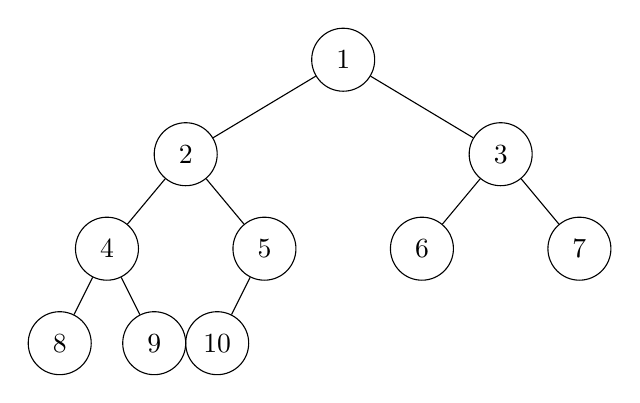
\begin{tikzpicture}[level distance=1.2cm,
      level 1/.style={sibling distance=4cm},
      level 2/.style={sibling distance=2cm},
      level 3/.style={sibling distance=1.2cm},
      every node/.style={circle, draw, minimum size=0.8cm}]
      \node {1}
        child {node {2}
          child {node {4}
            child {node {8}}
            child {node {9}}
          }
          child {
            node {5}
            child {node {10}}
            child[missing] % placeholder for right child of 5
          }
        }
        child {node {3}
          child {node {6}}
          child {node {7}}
        };
    \end{tikzpicture}
    \end{center}
    从上图可以看出,整体形态是一个三角形,但右下角(节点6和7的子节点位置)是缺失的。

\end{enumerate}

\textbf{其他选项分析:}
\begin{itemize}
    \item \textbf{A. 完整的三角形:} 这描述的是\textbf{满二叉树},满二叉树是完全二叉树的一种特例,但不能代表所有完全二叉树。
    \item \textbf{C. 缺左角的三角形:} 这直接违反了完全二叉树“最后一层节点靠左排列”的定义。
    \item \textbf{D. 底部呈锯齿状的三角形:} 这个描述不够准确。“缺右角”更精确地描述了其结构特征。
\end{itemize}
\end{solution}


\section*{191}
\begin{graybox}
完全二叉堆在物理上是向量,其所存储的元
素次序是:
A. 完全二叉树的先序遍历次序
B. 完全二叉树的中序遍历次序
C. 完全二叉树的后序遍历次序
D. 完全二叉树的层次遍历次序
\end{graybox}

\begin{solution}
正确答案是 D。

\textbf{详细分析:}

\begin{enumerate}
    \item \textbf{完全二叉堆的物理存储:}
    完全二叉堆通常使用一维数组(或向量)进行存储,这样做可以节省空间(不需要存储指针)并能方便地计算父子节点关系。

    \item \textbf{存储规则:}
    存储的方式是按照树的层次,从上到下,从左到右,依次将节点放入数组中。
    \begin{itemize}
        \item 树的根节点存储在数组的第一个位置(索引0或1)。
        \item 根节点的左孩子、右孩子紧随其后。
        \item 然后是下一层的所有节点,同样从左到右排列。
        \item ...以此类推。
    \end{itemize}
    例如,对于一个节点在数组索引 `i` 的位置(假设从0开始):
    \begin{itemize}
        \item 其左孩子在索引 `2*i + 1`
        \item 其右孩子在索引 `2*i + 2`
        \item 其父节点在索引 `(i-1) / 2`
    \end{itemize}

    \item \textbf{遍历次序分析:}
    \begin{itemize}
        \item \textbf{A. 先序遍历 (Pre-order):} 根 $\to$ 左子树 $\to$ 右子树。
        \item \textbf{B. 中序遍历 (In-order):} 左子树 $\to$ 根 $\to$ 右子树。
        \item \textbf{C. 后序遍历 (Post-order):} 左子树 $\to$ 右子树 $\to$ 根。
        \item \textbf{D. 层次遍历 (Level-order):} 从上到下逐层遍历,在同一层内从左到右遍历。
    \end{itemize}

    \item \textbf{结论:}
    通过比较可以发现,完全二叉堆在数组中的物理存储顺序,与对该树进行\textbf{层次遍历}得到的节点顺序是完全一致的。
\end{enumerate}
\end{solution}


\section*{192}
\begin{graybox}
在完全二叉堆中(大顶堆),不正确的
是
A. 任何节点的数值不超过其父亲
B. 兄弟节点之间的没有确定的大小关系
C. 节点的数值不超过其任何一个祖先
D. 整个堆中的最大元素在底部的叶子节点
\end{graybox}

\begin{solution}
不正确的是 D。

\textbf{详细分析:}

大顶堆(Max-Heap)是一种特殊的完全二叉树,它满足堆序性质:任何一个节点的值都大于或等于其子节点的值。

\begin{itemize}
    \item \textbf{A. 任何节点的数值不超过其父亲}
    这是大顶堆的基本定义。`child.value <= parent.value`。所以这个说法是\textbf{正确}的。

    \item \textbf{B. 兄弟节点之间的没有确定的大小关系}
    堆序性质只规定了父子节点之间的关系,但没有规定同一父节点的两个孩子(兄弟节点)之间的大小关系。例如,一个值为10的父节点,其子节点可以是(8, 5)也可以是(5, 8)。所以这个说法是\textbf{正确}的。

    \item \textbf{C. 节点的数值不超过其任何一个祖先}
    这是一个必然的推论。一个节点的值不超过其父亲,其父亲的值又不超过其祖父的值,以此类推,直到根节点。所以一个节点的值不会超过其路径上的任何一个祖先。这个说法是\textbf{正确}的。

    \item \textbf{D. 整个堆中的最大元素在底部的叶子节点}
    根据大顶堆的性质,最大的元素一定是位于\textbf{根节点}。因为根节点是所有节点的祖先,它的值大于或等于其他所有节点。所以这个说法是\textbf{错误}的。
\end{itemize}
\end{solution}

\section*{193}
\begin{graybox}
当前完全二叉堆物理上作为向量是\{10, 5,
8, 3, 2, 7\},插入新元素9后变为:
A. \{2, 3, 5, 7, 8, 9, 10\}
B. \{10, 9, 8, 7, 5, 3, 2\}
C. \{10, 5, 8, 3, 2, 7, 9\}
D. \{10, 5, 9, 3, 2, 7, 8\}
\end{graybox}

\begin{solution}
正确答案是 D。

\textbf{详细分析:}

插入操作分为两步:添加到末尾和上滤。
初始堆(大顶堆)为 `{10, 5, 8, 3, 2, 7}`。其树形结构为:
\begin{center}
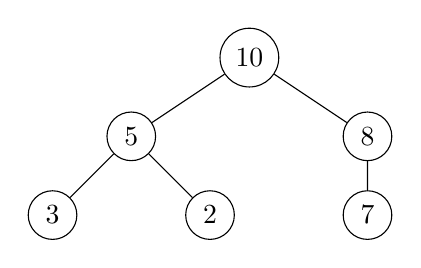
\begin{tikzpicture}[level distance=1cm,
  level 1/.style={sibling distance=3cm},
  level 2/.style={sibling distance=2cm},
  every node/.style={circle, draw}]
  \node {10}
    child {node {5}
      child {node {3}}
      child {node {2}}
    }
    child {node {8}
      child {node {7}}
    };
\end{tikzpicture}
\end{center}

\begin{enumerate}
    \item \textbf{添加到末尾:}
    将新元素 `9` 添加到向量的末尾,以维持完全二叉树的结构。
    向量变为:`{10, 5, 8, 3, 2, 7, 9}`。
    新元素 `9` 位于索引6的位置。

    \item \textbf{上滤(Percolate Up):}
    \begin{itemize}
        \item 新元素 `9` (在索引6) 的父节点是索引 `(6-1)/2 = 2` 的元素,即 `8`。
        \item 因为 `9 > 8`,违反了大顶堆的性质,所以需要将 `9` 和 `8` 交换。
        \item 交换后,向量变为:`{10, 5, 9, 3, 2, 7, 8}`。
        \item 元素 `9` 现在位于索引2。
    \end{itemize}
    \begin{itemize}
        \item 继续上滤。元素 `9` (在索引2) 的父节点是索引 `(2-1)/2 = 0` 的元素,即 `10`。
        \item 因为 `9 < 10`,满足大顶堆的性质,上滤过程结束。
    \end{itemize}
\end{enumerate}

最终,堆的向量表示为 \textbf{\{10, 5, 9, 3, 2, 7, 8\}}。
其树形结构为:
\begin{center}
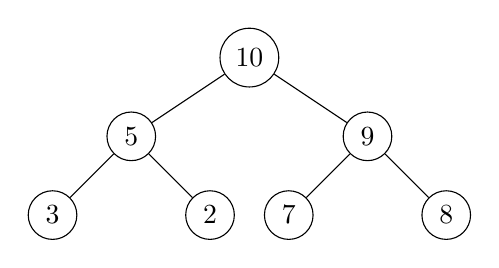
\begin{tikzpicture}[level distance=1cm,
  level 1/.style={sibling distance=3cm},
  level 2/.style={sibling distance=2cm},
  every node/.style={circle, draw}]
  \node {10}
    child {node {5}
      child {node {3}}
      child {node {2}}
    }
    child {node {9}
      child {node {7}}
      child {node {8}}
    };
\end{tikzpicture}
\end{center}
\end{solution}

\section*{194}
\begin{graybox}
当前完全二叉堆物理上作为向量是\{10,
5, 8, 3, 2, 7\},调用delMax()后变为:
A. \{5, 8, 3, 2, 7\}
B. \{2, 3, 5, 7, 8\}
C. \{8, 5, 7, 3, 2\}
D. \{8, 7, 5, 3, 2\}
\end{graybox}

\begin{solution}
正确答案是 C。

\textbf{详细分析:}

`delMax()` 操作(删除最大值)在大顶堆中分为三步:删除根节点、用最后一个元素替换根、下滤调整。
初始堆(大顶堆)为 `{10, 5, 8, 3, 2, 7}`。其树形结构为:
\begin{center}
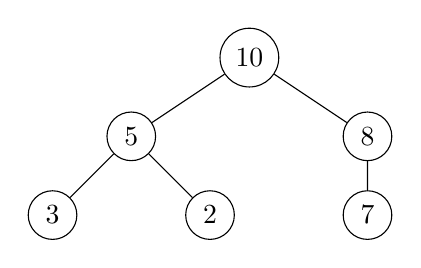
\begin{tikzpicture}[level distance=1cm,
  level 1/.style={sibling distance=3cm},
  level 2/.style={sibling distance=2cm},
  every node/.style={circle, draw}]
  \node {10}
    child {node {5}
      child {node {3}}
      child {node {2}}
    }
    child {node {8}
      child {node {7}}
    };
\end{tikzpicture}
\end{center}

\begin{enumerate}
    \item \textbf{删除根节点:}
    最大元素 `10`(根节点)被删除。

    \item \textbf{替换根节点:}
    将堆的最后一个元素 `7` 移动到根的位置,以维持完全二叉树的结构。
    此时向量变为 `{7, 5, 8, 3, 2}`。

    \item \textbf{下滤(Percolate Down):}
    \begin{itemize}
        \item 新的根节点 `7` (在索引0) 的子节点是 `5` (索引1) 和 `8` (索引2)。
        \item `7` 小于其较大的子节点 `8`,违反了大顶堆的性质。
        \item 将 `7` 与 `8` 交换。
        \item 交换后,向量变为:`{8, 5, 7, 3, 2}`。
        \item 元素 `7` 现在位于索引2。
    \end{itemize}
    \begin{itemize}
        \item 继续检查 `7`。它现在是叶子节点(其子节点索引将超出数组范围),因此满足堆序性。下滤过程结束。
    \end{itemize}
\end{enumerate}

最终,堆的向量表示为 \textbf{\{8, 5, 7, 3, 2\}}。
其树形结构为:
\begin{center}
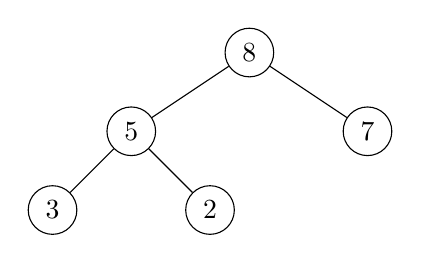
\begin{tikzpicture}[level distance=1cm,
  level 1/.style={sibling distance=3cm},
  level 2/.style={sibling distance=2cm},
  every node/.style={circle, draw}]
  \node {8}
    child {node {5}
      child {node {3}}
      child {node {2}}
    }
    child {node {7}};
\end{tikzpicture}
\end{center}
\end{solution}

\section*{195}
\begin{graybox}
现有n个元素需要组织成一个完全二叉堆,若
使用不断插入所有元素的方法,整个过程是:
A. 自上而下的上滤
B. 自上而下的下滤
C. 自下而上的上滤
D. 自下而上的下滤
\end{graybox}

\begin{solution}
正确答案是 A。

\textbf{详细分析:}

建堆有两种主要方法,题目描述的是其中一种。

\begin{enumerate}
    \item \textbf{方法描述:不断插入所有元素}
    \begin{itemize}
        \item 这个方法从一个空堆开始,逐一将 `n` 个元素插入。
        \item 每插入一个新元素,都将其放置在堆的末尾,然后执行一次\textbf{“上滤”(Percolate Up)}操作,将该元素与其父节点比较并可能交换,沿着路径向根节点方向移动,直到恢复堆序性。
    \end{itemize}

    \item \textbf{术语分析:}
    \begin{itemize}
        \item \textbf{上滤(Percolate Up):} 这是插入操作中使用的调整方法。因为元素是从下往上移动,所以这个操作本身是“自下而上”的。
        \item \textbf{下滤(Percolate Down):} 这是删除操作或Floyd建堆算法中使用的调整方法。元素是从上往下移动。
        \item \textbf{自上而下(Top-down) vs. 自下而上(Bottom-up):} 这两个词用来描述\textbf{整个建堆的策略}。
            \begin{itemize}
                \item \textbf{自上而下建堆:} 指的就是“不断插入”的方法。因为堆是从1个元素开始,逐渐增长到 `n` 个元素,概念上是从顶部开始构建并向下扩展。
                \item \textbf{自下而上建堆:} 指的是Floyd建堆算法(`heapify`)。它将整个数组视为一个乱序的树,从最后一个非叶子节点开始,向上逐个处理到根,对每个节点执行“下滤”。
            \end{itemize}
    \end{itemize}
\end{enumerate}

\textbf{结论:}
题目描述的“不断插入所有元素的方法”是\textbf{自上而下}的建堆策略,而该策略中每一步都使用\textbf{上滤}操作进行调整。因此,整个过程被称为“自上而下的上滤”。
\end{solution}

\section*{196}
\begin{graybox}
现有n个元素需要组织成一个完全二叉
堆,若使用Floyd算法,整个过程是:
A. 自上而下的上滤
B. 自上而下的下滤
C. 自下而上的上滤
D. 自下而上的下滤
\end{graybox}

\begin{solution}
正确答案是 D。

\textbf{详细分析:}

Floyd建堆算法,也称为`heapify`,是一种高效的批量建堆方法。

\begin{enumerate}
    \item \textbf{算法描述:}
    \begin{itemize}
        \item 该算法首先将 `n` 个元素视为一个完整的、但无序的完全二叉树。
        \item 它从最后一个\textbf{非叶子节点}开始,向前(即向数组的头部)遍历,直到根节点。
        \item 对于遍历到的每一个节点,算法都对其执行一次\textbf{“下滤”(Percolate Down)}操作。下滤操作会确保以当前节点为根的子树满足堆序性。
    \end{itemize}

    \item \textbf{术语分析:}
    \begin{itemize}
        \item \textbf{下滤(Percolate Down):} 这是Floyd算法中使用的核心调整方法。因为元素是从上往下移动以找到其正确位置。
        \item \textbf{自下而上(Bottom-up):} 这个词用来描述\textbf{整个建堆的策略}。因为算法是从最后一个非叶子节点(位于树的较底层)开始处理,然后逐层向上,最后处理根节点。所以整个建堆的宏观流程是“自下而上”的。
    \end{itemize}
\end{enumerate}

\textbf{结论:}
Floyd算法是一种\textbf{自下而上}的建堆策略,它在每一步都使用\textbf{下滤}操作进行调整。因此,整个过程被称为“自下而上的下滤”。
\end{solution}


\section*{197}
\begin{graybox}
堆排序在流程上类似于以前学过的哪种排序?
A. 选择排序
B. 插入排序
C. 冒泡排序
D. 归并排序
\end{graybox}

\begin{solution}
正确答案是 A。

\textbf{详细分析:}

\begin{enumerate}
    \item \textbf{选择排序(Selection Sort)的流程:}
    \begin{itemize}
        \item 在未排序的序列中,找到最大(或最小)的元素。
        \item 将该元素存放到已排序序列的末尾(或开头)。
        \item 重复以上步骤,直到所有元素均排序完毕。
    \end{itemize}
    选择排序的核心思想是:\textbf{每一次都从待排序的数据元素中选出最大(或最小)的一个元素},存放在序列的起始位置。

    \item \textbf{堆排序(Heap Sort)的流程:}
    \begin{itemize}
        \item 首先,将待排序的序列构建成一个大顶堆。
        \item 将堆顶元素(即当前序列中的最大值)与末尾元素交换。
        \item 将剩余的 `n-1` 个元素重新调整为一个大顶堆。
        \item 重复以上步骤,直到所有元素均排序完毕。
    \end{itemize}
    堆排序的核心思想也是:\textbf{每一次都从待排序的数据元素中选出最大(或最小)的一个元素}。

    \item \textbf{相似性对比:}
    两种排序算法的宏观流程是高度相似的,都是在每一轮中“选择”出当前未排序部分的最大(或最小)值,然后将其放置到正确的位置。

    \textbf{主要区别}在于“如何选择”最大值:
    \begin{itemize}
        \item \textbf{选择排序}通过线性扫描(遍历)来找到最大值,效率较低,每次选择的时间复杂度为 $O(n)$。
        \item \textbf{堆排序}通过维护堆的结构,使得每一次获取最大值的时间复杂度为 $O(1)$(即取堆顶),而后续调整堆的复杂度为 $O(\log n)$。因此,堆排序可以看作是选择排序的一种\textbf{优化版本}。
    \end{itemize}
\end{enumerate}
\end{solution}

\section*{198}
\begin{graybox}
堆排序的时间复杂度为:
A. O(n)
B. O(nlogn)
C. O(nlognlogn)
D. O(n\textsuperscript{2})
\end{graybox}

\begin{solution}
正确答案是 B。

\textbf{详细分析:}

堆排序(HeapSort)的整个过程可以分为两个主要阶段:

\begin{enumerate}
    \item \textbf{建堆(Heap Construction):}
    将一个包含 `n` 个元素的无序数组转换成一个大顶堆(或小顶堆)。
    \begin{itemize}
        \item 如果使用高效的Floyd建堆算法(`heapify`),这个阶段的时间复杂度为 $O(n)$。
        \item 如果使用逐个插入的方法建堆,这个阶段的时间复杂度为 $O(n \log n)$。
    \end{itemize}
    通常我们采用更高效的 $O(n)$ 方法。

    \item \textbf{排序(Sorting):}
    这个阶段循环 `n-1` 次,每次从堆中取出最大(或最小)的元素。
    \begin{itemize}
        \item 每次操作都是一次 `delMax`(或 `delMin`),包括将堆顶元素与末尾元素交换,并对新的堆顶进行“下滤”调整。
        \item “下滤”操作的时间复杂度与堆的高度成正比,即 $O(\log k)$,其中 `k` 是当前堆的大小。
        \item 这个过程需要执行 `n-1` 次,每次的成本分别是 $O(\log n), O(\log(n-1)), \dots, O(\log 2)$。
        \item 因此,这个阶段的总时间复杂度为 $\sum_{k=2}^{n} O(\log k) = O(n \log n)$。
    \end{itemize}
\end{enumerate}

\textbf{总时间复杂度:}
将两个阶段的复杂度相加:
$T(n) = T(\text{建堆}) + T(\text{排序}) = O(n) + O(n \log n)$

根据复杂度的加法规则,我们取增长率较高的项,所以堆排序的整体时间复杂度为 $O(n \log n)$。这个复杂度在最坏、平均和最好情况下都是一样的。
\end{solution}

\section*{199}
\begin{graybox}
堆排序的空间复杂度为:
A. O(1)
B. O(n)
C. O(nlogn)
D. O(n\textsuperscript{2})
\end{graybox}

\begin{solution}
正确答案是 A。

\textbf{详细分析:}

空间复杂度通常指的是算法在执行过程中所需要的\textbf{额外辅助空间},不包括存储输入数据本身所占用的空间。

\begin{enumerate}
    \item \textbf{堆排序的实现方式:}
    堆排序是一种\textbf{原地排序(in-place sorting)}算法。这意味着它不需要一个与原始数组同样大小的额外数组来存储数据。所有的排序操作,包括建堆和排序阶段的元素交换,都是在原始输入数组上直接进行的。

    \item \textbf{空间使用情况:}
    \begin{itemize}
        \item 在整个排序过程中,算法只需要有限的几个临时变量来存储索引或在交换元素时暂存数据。
        \item 例如,在交换堆顶和末尾元素时,需要一个临时变量 `temp`。
        \item 这种所需额外空间的数量是固定的,不随待排序数组的规模 `n` 的增长而增长。
    \end{itemize}

    \item \textbf{结论:}
    由于堆排序只需要常数级别的额外空间,其空间复杂度为 $O(1)$。
\end{enumerate}

\textbf{注意:}
如果堆排序中的“下滤”操作使用递归来实现,那么会产生递归调用栈的开销。这个栈的深度最大为堆的高度,即 $O(\log n)$。但在通常的讨论中,堆排序指的是其迭代实现,并且被归类为空间复杂度为 $O(1)$ 的原地排序算法。
\end{solution}






\end{document}

% VScode 常用快捷键:

% Ctrl + R:                 打开最近的文件夹
% F2:                       变量重命名
% Ctrl + Enter:             行中换行
% Alt + up/down:            上下移行
% 鼠标中键 + 移动:           快速多光标
% Shift + Alt + up/down:    上下复制
% Ctrl + left/right:        左右跳单词
% Ctrl + Backspace/Delete:  左右删单词    
% Shift + Delete:           删除此行
% Ctrl + J:                 打开 VScode 下栏(输出栏)
% Ctrl + B:                 打开 VScode 左栏(目录栏)
% Ctrl + `:                 打开 VScode 终端栏
% Ctrl + 0:                 定位文件
% Ctrl + Tab:               切换已打开的文件(切标签)
% Ctrl + Shift + P:         打开全局命令(设置)

% Latex 常用快捷键

% Ctrl + Alt + J:           由代码定位到PDF
% 


% Git提交规范:
% update: Linear Algebra 2 notes
% add: Linear Algebra 2 notes
% import: Linear Algebra 2 notes
% delete: Linear Algebra 2 notes
